\section{Smart Governance}

%Wie ist der Stand bei Smart Governance in Hamburg?
Um das Ziel der Smart Governance in einer Stadt zu erreichen, sollte sie mit Fokus auf vier grundlegende Dimensionen umgestaltet werden.
\begin{enumerate}
	\item Smarte Regierung
	\item Offene \& verknüpfte Daten
	\item Digitaler Service \& kooperative Regierung
	\item Stadtinfrastruktur
\end{enumerate}
\autocite[14]{Fuetterer.2020}
\\ Quantitativ sind diese Dimensionen bereits mit Projekten befüllt. Im Portal \glqq Smart City Kompass\grqq\space werden in ganz Hamburg mehr Smart-Governance-Projekte durchgeführt als in jeder anderen deutschen Stadt \autocite{SmartCityKompass.2020}. Um die Qualität dieser Projekte herauszufinden, werden zwei der Projekte exemplarisch detailliert untersucht und evaluiert.
\\ Im Jahr 2012 verabschiedete die hamburger Regierung ein neuartiges Gesetz, das zu einem Grundpfeiler für die Weiterentwicklung von Open-Government-Initiativen nicht nur in Hamburg sondern auch in vielen anderen Städten Deutschlands werden sollte. Das Ziel des Gesetzes war es, Informationen aus der Senatsarbeit der Allgemeinheit unmittelbar zugänglich zu machen \autocite{Senat.2012}. Die Regelungen in diesem Gesetz wurden umgesetzt mithilfe einer neu entwickelten Online-Plattform, dem \glqq Transparenzportal\grqq.
\\ Diese frei zugängliche Website ermöglicht es jedem Bürger aus Hamburg, aber auch aus allen anderen Bereichen der Erde, Daten aus der hamburger Senatsarbeit frei einzusehen. Abbildung \ref{fig:3_transparenzportal} zeigt beispielhaft die verfügbaren Datensätze wenn Bürger nach Daten zum Bauprojekt der Elbphilharmonie suchen.

\begin{figure}
	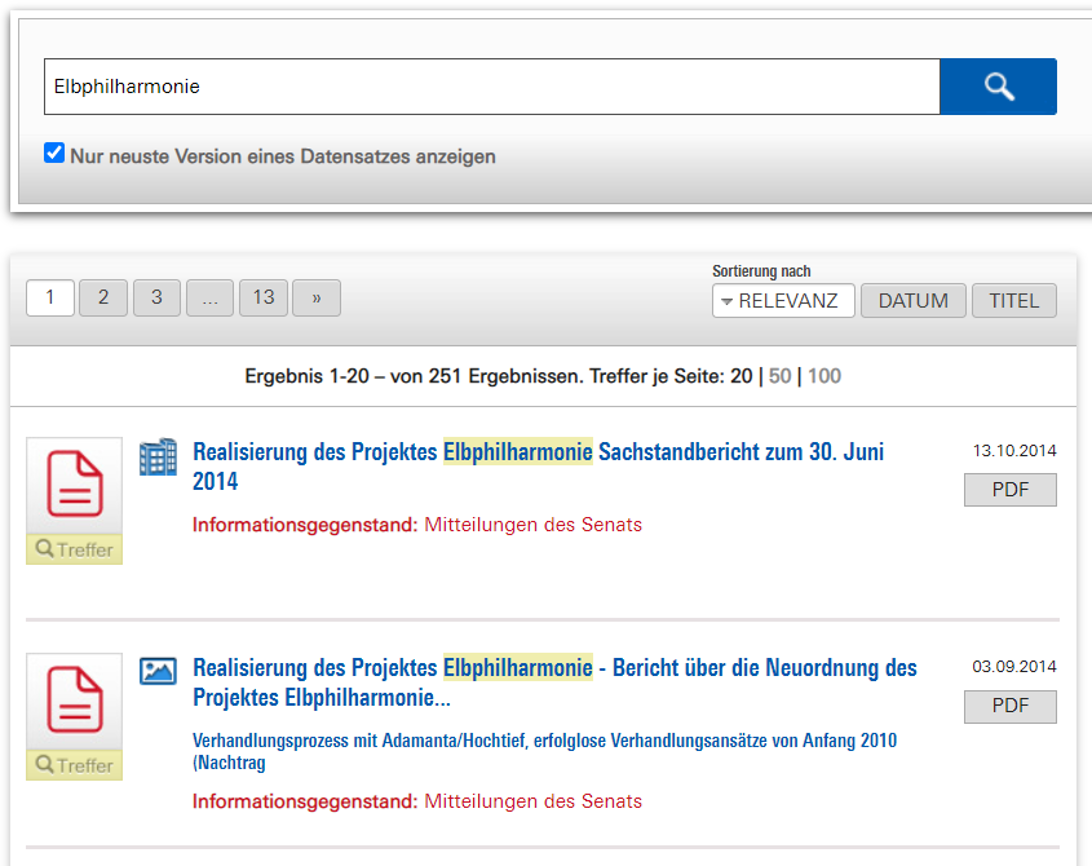
\includegraphics[width=\textwidth]{graphics/3-transparenzportal}
	\caption[Suchergebnisse im Transparenzportal Hamburg]{Suchergebnisse im Transparenzportal Hamburg}
	\label{fig:3_transparenzportal}
\end{figure}

%Welche Beispielprojekte belegen dass?

%Auf welchem Weg ist Hamburg auf dem Weg zur Smart City im Bereich der Smart Governance?


%- Aspekte Smart Governance (laut Smart City Wheel):
%  - Stadtinfrastruktur
%  - digitaler Servide und kooperative Regierung
%  - offene und verknüpfte Daten
%  - Smarte Regierung
%- Open Government
%  - Open Government sollte seine Daten (Gov Data) offen legen (Open Data)
%- Interaktion zwischen Bevölkerung und Regierung soll durch "Open Government Data" befördert werden
%- Definition "Offene Daten"
%  - Verfügbarkeit (in zweckmäßiger Form und zu möglichst niedrigen Kosten)
%  - Wiederverwendung (daten müssen (auch maschinell) verarbeitbar sein)
%  - Universelle Beteiligung (Nutzung jeder Person ermöglicht)
%-  Ziele, um Open Government zu erreichen
%  - Transparenz
%  - Beteiligung
%  - Zusammenarbeit